%
% File acl2017.tex
%
%% Based on the style files for ACL-2015, with some improvements
%%  taken from the NAACL-2016 style
%% Based on the style files for ACL-2014, which were, in turn,
%% based on ACL-2013, ACL-2012, ACL-2011, ACL-2010, ACL-IJCNLP-2009,
%% EACL-2009, IJCNLP-2008...
%% Based on the style files for EACL 2006 by 
%%e.agirre@ehu.es or Sergi.Balari@uab.es
%% and that of ACL 08 by Joakim Nivre and Noah Smith

\documentclass[11pt,a4paper]{article}
\usepackage[hyperref]{acl2017}
\usepackage{times}
\usepackage{latexsym}
\usepackage{graphicx}
\usepackage{booktabs}
\usepackage{amsmath}
\usepackage{todonotes}
\usepackage{multirow}
\usepackage{enumitem}
\usepackage{amsfonts}
\usepackage{url}

\makeatletter
\newcommand{\@emptybiblabel}[1]{}
\makeatother
\DeclareMathOperator*{\argmax}{arg\,max}
\setlength\titlebox{3.5cm}    % Expanding the titlebox

\newcommand*{\checktikz}[1][]{\tikz[x=1em, y=1em]\fill[#1] (0,.35) -- (.25,0) -- (1,.7) -- (.25,.15) -- cycle;}
\newcommand*{\crosstikz}[1][]{\tikz[x=1em, y=1em]\fill[#1] (0,0) -- (1,1) -- (0.5,0.5) -- (0.1,0.1) -- cycle;}

\aclfinalcopy % Uncomment this line for the final submission

\newcommand\BibTeX{B{\sc ib}\TeX}
\newcommand{\Correct}{\checktikz[draw=black]}
\newcommand{\ValidMiss}{\checktikz[draw=gray,fill=white]}
\newcommand{\Valid}{\checktikz[draw=gray,fill=white]}
\newcommand{\Missed}{\checktikz[draw=black]} %\textsf{X}~}
\newcommand{\Wrong}{} %\textsf{X}~}

\newcommand{\U}{\mathbb{U}}

\title{Are you asking the right questions? \\ Automatically Generating Clarification Questions}
\author{ 
  \textbf{Sudha Rao}${}^{1}$\textnormal{,} \textbf{Hal Daum\'e III}${}^{1,3}$\\
  ${}^1$Computer Science,
  ${}^2$UMIACS\\
  University of Maryland\\
  raosudha@cs.umd.edu, hal@cs.umd.edu
  }

\date{}

\begin{document}
\maketitle
Inquiry is fundamental to communication, and machines cannot effectively collaborate with humans unless they can ask questions. In this work, we explore how can a machine automatically generate clarification questions when faced with uncertainty, a task of increasing importance in today's automated society. 
A main goal of asking questions is to fill information gaps, typically through clarification questions, which naturally occur in conversations. 
A good question is one whose \emph{likely answer} is going to be most useful.
We study the problem of question generation using data from StackExchange, a plentiful online resource in which people routinely ask clarifying questions to posts so that they can better offer assistance to the original poster. Consider the exchange in Figure~\ref{askubuntu_post}, in which an initial poster (who we'll call ``Terry'') asks for help configuring environment variables.
This question is underspecified and a responder (``Parker'') asks a clarifying question ``\textsf{\small What version of Ubuntu do you have?}''
Our goal in this work is to automate Parker.
Specifically, after Terry writes their initial post, we aim to generate a clarification question so that Terry can immediately amend their post in hopes of getting faster and better replies.
%
Our work has two main contributions: 
\begin{enumerate}[noitemsep,nolistsep]
	\item A novel neural-network model for addressing this task that integrates the notion of expected value of perfect information. 
	\item A novel dataset, derived from StackExchange, that enables us to learn a model to ask clarifying questions by looking at the types of questions people ask 
\end{enumerate}

In order to choose what question to ask, we build a neural network model inspired by the theory of expected value of perfect information (EVPI). EVPI is a measurement of: if I were to acquire information X, how useful would that be to me? However, because we haven't acquired X yet, we have to take this quantity in expectation over all possible X, weighted by each X's likelihood. In the question generation setting, for any given question $q$, there is set $A$ of possible answers. For each possible answer $a \in A$, there is some probability of getting that answer, and some utility if that were the answer we got. The theory of EVPI then states that we want to choose the question $q$ that maximizes:
\begin{equation}\label{evpi_equation}
\argmax_{q \in Q} \sum_{a \in A} \mathbb{P}[a | p,q] \U(p+a)
\end{equation} 
\begin{figure}[!t]
	\centering
	\setlength\fboxsep{1pt}
	\setlength\fboxrule{0.5pt}
	\fbox{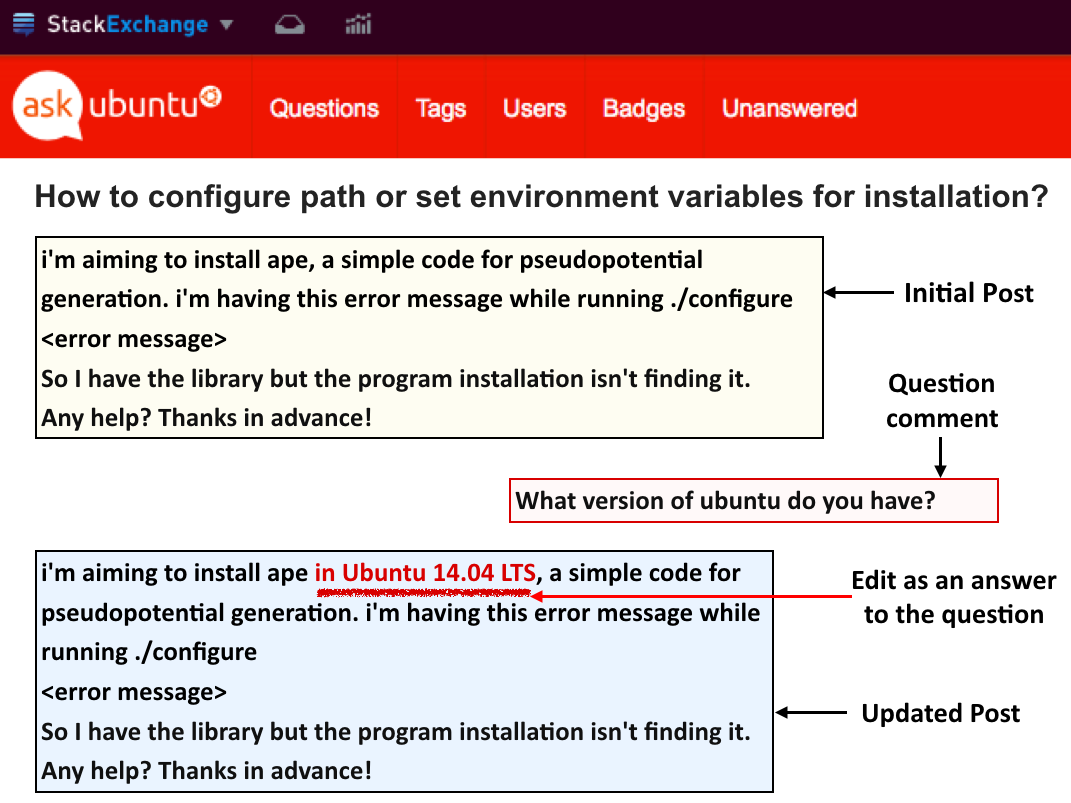
\includegraphics[width=0.47\textwidth]{askubuntu_post}}
	\caption{A post on an online Q \& A forum ``askubuntu.com'' is updated to fill the missing information pointed out by the question comment}
	\label{askubuntu_post}
\end{figure}


$\mathbb{P}[a | p,q]$ measures the probability of getting an answer $a$ given an initial post $p$ and a clarifying question $q$. $\U(p+a)$ is a utility function that measures how useful it would be if $p$ were augmented with answer $a$. We represent both our probability distribution model $\mathbb{P}$ and our utility function $U$ using neural networks over the appropriate inputs.  We train the parameters of the two models jointly to minimize a joint loss defined such that an answer that has a higher potential of increasing the utility of a post gets a higher probability. We train our model using $(p,q,a)$ triples that we extract automatically using StackExchange's edit history. In the figure, we extract the initial post as $p$, question posted in the comments section as $q$, and edit to the original post as answer $a$. Our results show significant improvements from using the EVPI formalism over both standard feedforward network architectures and bag-of-ngrams baselines.

\bibliography{acl2017}
\bibliographystyle{acl_natbib}

\end{document}
